\index{numerical integration}
\index{stochastic gradient descent}
\chapter{Numerical Integration}
\printchapterversion{6_integration_and_sgd}
\newthought{Smooth Operator.}


% ==============================================================================================
% INTRODUCTION BLOCK

\section{The Why}
\index{numerical integration!motivation}

\marginnote{\newthought{Melts all your memories} \href{https://open.spotify.com/track/1Hv1VTm8zeOeybub15mA2R?si=2b063718fca34b6a}{ and change into gold}}

\newthought{In the previous chapter,} we explored global optimization strategies to escape local minima.
Imagine you are optimizing a function with thousands of tiny, sharp local minima like a high-frequency version of Shekel’s Foxholes. 
A gradient descent algorithm will get stuck instantly in the first microscopic pothole it finds.


\newthought{The solution for this} is one that will feel familiar, but probably did go unnoticed until now: Numerical integration. 
\begin{equation}
    I = \int_a^b f(x) \, dx
\end{equation}

\newthought{This gives us good reasons} to understand numerical integration,
\begin{itemize}
    \item as it allows us to smoothen the loss landscape and make optimization methods more robust.
    \item as it tends to find more robust optima due to the averaging effect\cite{batchtraining} of a region.
\end{itemize}


\newthought{In deep learning} stochastic gradient descent (SGD) is the workhorse optimization algorithm.

\marginnote{\newthought{Monte Carlo} is a strategy which basically solves problems by random sampling. Embrace the beauty: }

It is a Monte Carlo\cite{randomsearch}\cite{montecarlodropout} method that estimates the gradient of the loss function by averaging over the gradient of a 
random mini-batch of data points. We are lucky to have numerical integration around, as it would be prohibitive expensive to train models on large-scale datasets.









\newpage
\subsection{Hands On Experience}
\index{numerical integration!hands-on}
\index{discretization} \index{approximation} \index{stepsize} \index{interval}

We already know how to discretize a continuous function, and how to handle finite precision and systems with sparse information at discrete points.


\begin{figure}[h]
    \centering
    % Requires: \usepackage{pgfplots}
    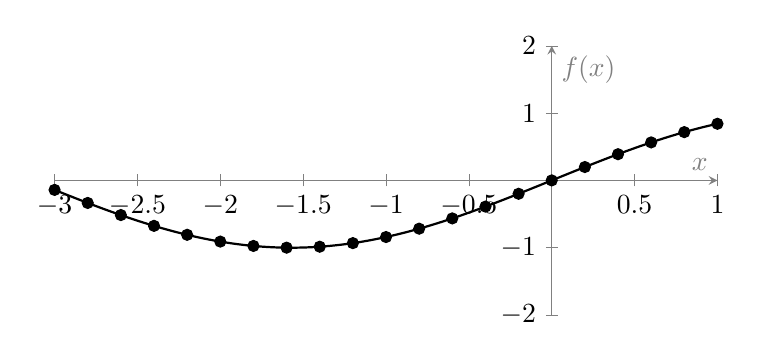
\begin{tikzpicture}
        \begin{axis}[
              width=10cm,
              height=5cm,
              axis x line=middle,
              axis y line=middle,
              xlabel={$x$},
              ylabel={$f(x)$},
              domain=-3:1,
              samples=100,
              ymin=-2, ymax=2,
              xmin=-3, xmax=1,
              legend style={at={(0.5,-0.2)},anchor=north},
              tick style={gray},
              label style={gray},
              axis line style={gray},
        ]
        % Continuous curve
        \addplot[black, thick, smooth] {sin(deg(x))};
        % Discretized points every 0.2 from -3 to 1
        \addplot[black, only marks, mark=*] coordinates {
            (-3.0, -0.1411)
            (-2.8, -0.33499)
            (-2.6, -0.51504)
            (-2.4, -0.67546)
            (-2.2, -0.80850)
            (-2.0, -0.90930)
            (-1.8, -0.97385)
            (-1.6, -0.99957)
            (-1.4, -0.98545)
            (-1.2, -0.93204)
            (-1.0, -0.84147)
            (-0.8, -0.71736)
            (-0.6, -0.56464)
            (-0.4, -0.38942)
            (-0.2, -0.19867)
            (0.0, 0.0)
            (0.2, 0.19867)
            (0.4, 0.38942)
            (0.6, 0.56464)
            (0.8, 0.71736)
            (1.0, 0.84147)
        };
        \end{axis}
    \end{tikzpicture}
    \caption{Continuous curve $f(x) = \sin(x)$ and its discretized version (black dots) on $[-3,1]$ with step size $h=0.2$.}
    \label{fig:discretizationlowfrequency}
\end{figure}

\newthought{The Shekel function}, as a high-frequency function, did pose a challenge for global optimization, yet did not render our general approaches obsolete. We still discretize and treat these functions as we are used to.

\begin{figure}[h]
    \centering
    % Requires: \usepackage{pgfplots}
    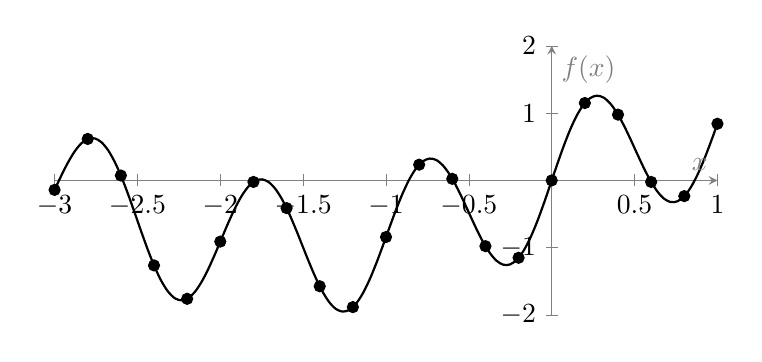
\begin{tikzpicture}
        \begin{axis}[
              width=10cm,
              height=5cm,
              axis x line=middle,
              axis y line=middle,
              xlabel={$x$},
              ylabel={$f(x)$},
              domain=-3:1,
              samples=100,
              ymin=-2, ymax=2,
              xmin=-3, xmax=1,
              legend style={at={(0.5,-0.2)},anchor=north},
              tick style={gray},
              label style={gray},
              axis line style={gray},
        ]
        % Continuous curve: sum of sin(x) and sin(2πx)
        \addplot[black, thick, smooth] {sin(deg(x)) + sin(360*x)};
        % Discretized points every 0.2 from -3 to 1 for f(x)=sin(x)+sin(2\pi x)
        \addplot[black, only marks, mark=*] coordinates {
            (-3.0, -0.14112)
            (-2.8, 0.61607)
            (-2.6, 0.07275)
            (-2.4, -1.26325)
            (-2.2, -1.75955)
            (-2.0, -0.90930)
            (-1.8, -0.02279)
            (-1.6, -0.41179)
            (-1.4, -1.57323)
            (-1.2, -1.88310)
            (-1.0, -0.84147)
            (-0.8, 0.23370)
            (-0.6, 0.02314)
            (-0.4, -0.97720)
            (-0.2, -1.14973)
            (0.0, 0.0)
            (0.2, 1.14973)
            (0.4, 0.97720)
            (0.6, -0.02314)
            (0.8, -0.23370)
            (1.0, 0.84147)
        };
        \end{axis}
    \end{tikzpicture}
    \caption{Continuous curve $f(x)=\sin(x)+\sin(2\pi x)$ and its discretized version (black dots) on $[-3,1]$ with step size $h=0.2$.}
    \label{fig:discretizationhighfrequency}
\end{figure}

\newthought{Taking a closer look at any} local minima shows how the high-frequency loss landscape will nudge our optimization algorithm into the nearest local minimum.
For example at $x=0.6$ or $x=-0.4$.

\begin{figure}[h]
    \centering
    % Requires: \usepackage{pgfplots}
    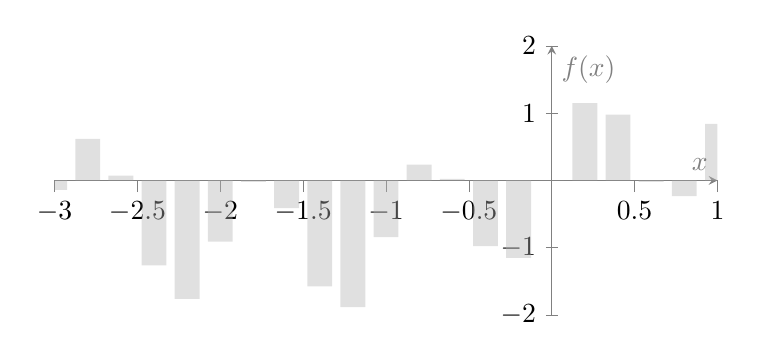
\begin{tikzpicture}
        \begin{axis}[
              width=10cm,
              height=5cm,
              axis x line=middle,
              axis y line=middle,
              xlabel={$x$},
              ylabel={$f(x)$},
              domain=-3:1,
              samples=100,
              ymin=-2, ymax=2,
              xmin=-3, xmax=1,
              legend style={at={(0.5,-0.2)},anchor=north},
              tick style={gray},
              label style={gray},
              axis line style={gray},
              ybar,
              bar width=0.15,
        ]
        % Bar plot for discretized summed values (h=0.2)
        \addplot[fill=gray!60, fill opacity=0.4, draw=none] coordinates {
            (-3.0, -0.14112)
            (-2.8, 0.61607)
            (-2.6, 0.07275)
            (-2.4, -1.26325)
            (-2.2, -1.75955)
            (-2.0, -0.90930)
            (-1.8, -0.02279)
            (-1.6, -0.41179)
            (-1.4, -1.57323)
            (-1.2, -1.88310)
            (-1.0, -0.84147)
            (-0.8, 0.23370)
            (-0.6, 0.02314)
            (-0.4, -0.97720)
            (-0.2, -1.14973)
            (0.0, 0.0)
            (0.2, 1.14973)
            (0.4, 0.97720)
            (0.6, -0.02314)
            (0.8, -0.23370)
            (1.0, 0.84147)
        };
        \end{axis}
    \end{tikzpicture}
    \caption{Continuous curve $f(x)=\sin(x)+\sin(2\pi x)$ and its discretized version (black dots) on $[-3,1]$ with step size $h=0.2$.}
    \label{fig:discretizationhighfrequency}
\end{figure}



\newthought{Consider approximation by numerical integration.} Let's see what it does at $x=-0.4$, instead of 
solving directly for: 

\begin{equation}
    f(-0.4) = -0.97720,
\end{equation}

let's approximate the value through integration with width \\ $h=0.2$:

\begin{align*}
    h \cdot f(-0.4) &\approx \int_{-0.5}^{-0.3} f(x) \, dx \\ 
            &\approx \frac{h}{2}[f(-0.5) + f(-0.3)] \\
            &\approx 0.2 \cdot \frac{-1.14973 - 0.97720}{2} \\
            &= -0.11285
\end{align*}
\begin{align*}
    f(-0.4) &\approx \frac{-1.14973 - 0.97720}{2} \\
            &= -1.06347
\end{align*}

\newthought{This is a much better approximation} having global optima in mind, than the direct evaluation at $x=-0.4$ which gave us $-0.97720$.
The numerical integration gave us a correction of the local loss landscape towards higher losses at this local minima.
The next figure shows the effect of this smoothing on the whole curve.

\begin{figure}[h]
    \centering
    % Requires: \usepackage{pgfplots}
    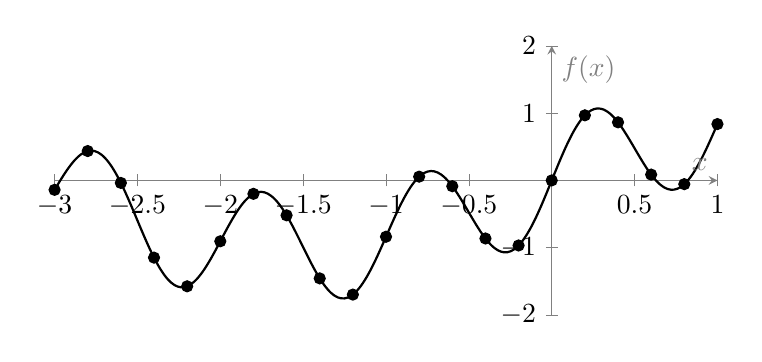
\begin{tikzpicture}
        \begin{axis}[
              width=10cm,
              height=5cm,
              axis x line=middle,
              axis y line=middle,
              xlabel={$x$},
              ylabel={$f(x)$},
              domain=-3:1,
              samples=100,
              ymin=-2, ymax=2,
              xmin=-3, xmax=1,
              legend style={at={(0.5,-0.2)},anchor=north},
              tick style={gray},
              label style={gray},
              axis line style={gray},
        ]
        % Smoothed continuous curve: average of neighbours at ±h/2 (h=0.2 → ±0.1)
        \addplot[black, thick, smooth, domain=-3:1, samples=200] {((sin(deg(x-0.1)) + sin(360*(x-0.1)) + sin(deg(x+0.1)) + sin(360*(x+0.1)))/2)};
        % Smoothed discretized points every 0.2 from -3 to 1 using the same neighbour-average
        \addplot[black, only marks, mark=* , samples at={-3.0,-2.8,-2.6,-2.4,-2.2,-2.0,-1.8,-1.6,-1.4,-1.2,-1.0,-0.8,-0.6,-0.4,-0.2,0.0,0.2,0.4,0.6,0.8,1.0}] {((sin(deg(x-0.1)) + sin(360*(x-0.1)) + sin(deg(x+0.1)) + sin(360*(x+0.1)))/2)};
        \end{axis}
    \end{tikzpicture}
    \caption{Continuous curve $f(x)=\sin(x)+\sin(2\pi x)$ and its discretized version (black dots) on $[-3,1]$ with step size $h=0.2$, and smoothed by numerical integration with interval length $h$.}
    \label{fig:discretizationhighfrequencysmoothed}
\end{figure}

\newthought{The smoothing} becomes even more apparent when integrating over larger intervals in general, or in our engineered example when choosing $h$ such that the frequency of the noisy signal gets averaged out.

\marginnote{\newthought{What if,} we would be integrating over an interval which results in destructive inference of the underlying higher frequency sine curve? Think wavelengths.}

\begin{figure}[h]
    \centering
    % Requires: \usepackage{pgfplots}
    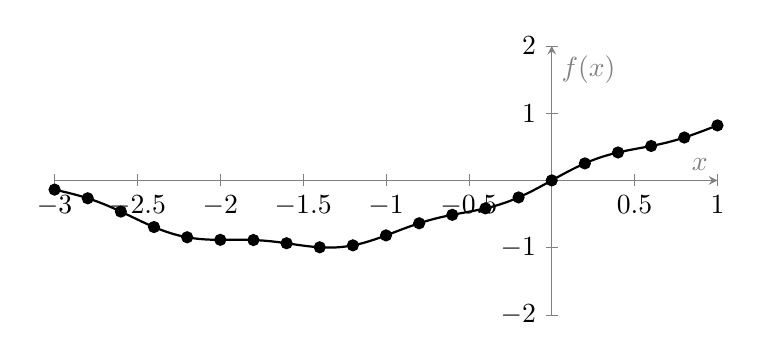
\begin{tikzpicture}
        \begin{axis}[
              width=10cm,
              height=5cm,
              axis x line=middle,
              axis y line=middle,
              xlabel={$x$},
              ylabel={$f(x)$},
              domain=-3:1,
              samples=100,
              ymin=-2, ymax=2,
              xmin=-3, xmax=1,
              legend style={at={(0.5,-0.2)},anchor=north},
              tick style={gray},
              label style={gray},
              axis line style={gray},
        ]
        % Smoothed continuous curve: average of neighbours at ±h/2 (choose h=0.48 → ±0.24 to get close to cancel sin(2\pi x))
        \addplot[black, thick, smooth, domain=-3:1, samples=200] {((sin(deg(x-0.24)) + sin(360*(x-0.24)) + sin(deg(x+0.24)) + sin(360*(x+0.24)))/2)};
        % Smoothed discretized points every 0.2 from -3 to 1 using the same neighbour-average
        \addplot[black, only marks, mark=* , samples at={-3.0,-2.8,-2.6,-2.4,-2.2,-2.0,-1.8,-1.6,-1.4,-1.2,-1.0,-0.8,-0.6,-0.4,-0.2,0.0,0.2,0.4,0.6,0.8,1.0}] {((sin(deg(x-0.24)) + sin(360*(x-0.24)) + sin(deg(x+0.24)) + sin(360*(x+0.24)))/2)};
        \end{axis}
    \end{tikzpicture}
    \caption{Continuous curve $f(x)=\sin(x)+\sin(2\pi x)$ and its discretized version (black dots) on $[-3,1]$ with step size $h=0.2$, smoothed by neighbour averaging with $h=0.48$ (so $h/2=0.24$ gets close to cancel the $\sin(2\pi x)$ component).}
    \label{fig:discretizationhighfrequencysmoothedOne}
\end{figure}

\newthought{While you have} seen the smoothing effect driven by the interval size, the approximation of the interval so far is a pretty coarse approximation, relying on two points only.

\vspace{2.5em}
\newthought{The Learning Objectives} of this chapter will provide you with the abilities to:
\begin{itemize}
    \item Derive and apply the midpoint method, trapezoid and Simpson's rules for numerical integration
    \item Understand composite rules for improved accuracy
    \item Know about Lagrange interpolation and how it relates to quadrature rules
    \item Understand how the curse of dimensionality motivates Monte Carlo 
    \item Derive and apply Monte Carlo integration for high-dimensional problems
    \item Apply Monte Carlo integration and recognize that batch averaging in ML is numerical integration
\end{itemize}








% ==============================================================================================
% MAIN THEORY BLOCK

\newpage
\subsection{Methods of Numerical Intgration}
\vspace{1em}

\newthought{The most trivial approximation of integrals} is using a single discretized value. 


\begin{align*}
    I &= \int_a^b f(x)\, dx. \\ 
    I &= \frac{b-a}{n} \cdot f\left(\frac{a+b}{2}\right) \\
    I &= h \cdot f(m)
\end{align*}

It is easy to see that the height of the rectangle is the value at the midpoint, and the width is $h$.

We can further refine the approximation of the integral by dividing $[a, b]$ into $n$ subintervals of equal width $h$, and summing the contributions from each interval.
This is also known as Riemann sum approximation, and can be expressed as:
\begin{align*}
    \int_a^b f(x)\, dx &\approx \sum_{i=0}^{n-1} \int_{x_i}^{x_{i+1}} f(x)\, dx \\
    &\approx \sum_{i=0}^{n-1} h \cdot f(m_i) \\
\end{align*}
where $x_i = a + i h$ for $i = 0, 1, \ldots, n$.

\marginnote{\newthought{On the interval $[a, b]$}, the midpoint value is $f(m)$. With left endpoint, the height is $f(a)$; with right endpoint, the height is $f(b)$.}

\newthought{The midpoint rule} of these composite intervals uses the midpoint, which is the average of the endpoints, of each interval, 
which often gives better results than left or right endpoint methods. Intuitively, this is because the midpoint approximates the curvature of the function better on the interval.

\begin{figure}[h]
    \centering
    % Requires: \usepackage{pgfplots}
    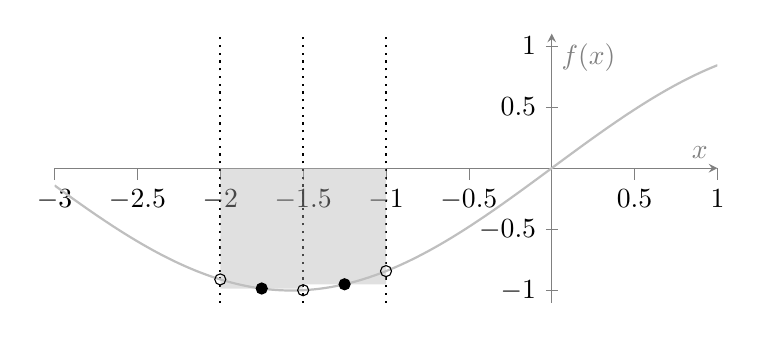
\begin{tikzpicture}
        \begin{axis}[
              width=10cm,
              height=5cm,
              axis x line=middle,
              axis y line=middle,
              xlabel={$x$},
              ylabel={$f(x)$},
              domain=-3:1,
              samples=100,
              ymin=-1.1, ymax=1.1,
              xmin=-3, xmax=1,
              legend style={at={(0.5,-0.2)},anchor=north},
              tick style={gray},
              label style={gray},
              axis line style={gray},
              ybar,
              bar width=0.5,
        ]
                % Vertical dotted guide lines (use axis coordinates to avoid interfering with plots)
                    \draw[dotted, thick, black] (axis cs:-2,-1.1) -- (axis cs:-2,1.1);
                    \draw[dotted, thick, black] (axis cs:-1.5,-1.1) -- (axis cs:-1.5,1.1);
                    \draw[dotted, thick, black] (axis cs:-1,-1.1) -- (axis cs:-1,1.1);
        % Gray bars for midpoint rule intervals (no gap)
        \addplot[fill=gray!60, fill opacity=0.4, draw=none] coordinates {
            (-1.75, -0.98363)
            (-1.25, -0.94898)
        };
        % Continuous curve: sin(x) in light gray
        \addplot[gray!50, thick, smooth] {sin(deg(x))};
        % Discretized points at midpoints
        \addplot[black, only marks, mark=*] coordinates {
            (-1.75, -0.98363)
            (-1.25, -0.94898)
        };
        % Discretized points at endpoints
        \addplot[black, only marks, mark=o] coordinates {
            (-2, -0.90930)
            (-1.5, -0.99749)
            (-1, -0.84147)
        };
        \end{axis}
    \end{tikzpicture}
    \caption{Continuous curve $f(x)=\sin(x)$ and midpoint rule integrals (gray bars) for $a=-2$, $b=-1$, $h=0.5$. Black dots: midpoints. Circles: endpoints.
    The bars now touch, illustrating the midpoint rule without a gap.}
    \label{fig:midpointrule}
\end{figure}


\newthought{Increasing the number of subintervals} reduces the error.
\marginnote{\newthought{Doubling the sub intervals} reduced error by $\sim 4\times$. This suggests $O(h^2)$ convergence.}
This of course comes at the cost of more function evaluations, and thus more computational cost. So can we do better than approximating midpoints? 





\newthought{Trapezoids} are more expressive geometrically than rectangles, and can capture linear 
changes in the function between the endpoints.

% Trapezoid rule for a single interval [a, b]
\begin{equation}
    \int_a^b f(x)\, dx \approx \frac{h}{2}\left[f(a) + f(b)\right]
\end{equation}
where $h = b - a$.


\begin{figure}[h]
    \centering
    % Requires: \usepackage{pgfplots}
    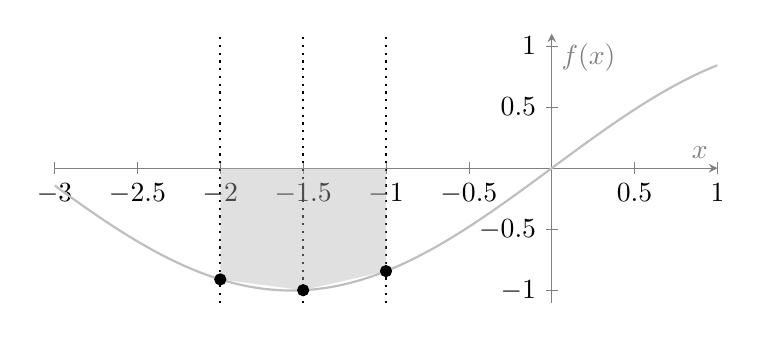
\begin{tikzpicture}
        \begin{axis}[
              width=10cm,
              height=5cm,
              axis x line=middle,
              axis y line=middle,
              xlabel={$x$},
              ylabel={$f(x)$},
              domain=-3:1,
              samples=100,
              ymin=-1.1, ymax=1.1,
              xmin=-3, xmax=1,
              legend style={at={(0.5,-0.2)},anchor=north},
              tick style={gray},
              label style={gray},
              axis line style={gray},
        ]
          % Vertical dotted lines at x=-2, -1.5, -1
          \addplot[dotted, thick, black, domain=-2:-2, samples=2] coordinates {(-2,-1.1) (-2,1.1)};
          \addplot[dotted, thick, black, domain=-1.5:-1.5, samples=2] coordinates {(-1.5,-1.1) (-1.5,1.1)};
          \addplot[dotted, thick, black, domain=-1:-1, samples=2] coordinates {(-1,-1.1) (-1,1.1)};
        % Continuous curve: sin(x) in light gray
        \addplot[gray!50, thick, smooth] {sin(deg(x))};
        % Trapezoids for intervals [-2,-1.5] and [-1.5,-1]
        \addplot [
            fill=gray!60, fill opacity=0.4, draw=none
        ] coordinates {
            (-2, -0.90930)
            (-1.5, -0.99749)
            (-1.5, 0)
            (-2, 0)
            (-2, -0.90930)
        };
        \addplot [
            fill=gray!60, fill opacity=0.4, draw=none
        ] coordinates {
            (-1.5, -0.99749)
            (-1, -0.84147)
            (-1, 0)
            (-1.5, 0)
            (-1.5, -0.99749)
        };
        % Endpoints
        \addplot[black, only marks, mark=*] coordinates {
            (-2, -0.90930)
            (-1.5, -0.99749)
            (-1, -0.84147)
        };
        \end{axis}
    \end{tikzpicture}
    \caption{Continuous curve $f(x)=\sin(x)$ and trapezoid rule areas (gray trapezoids) for $a=-2$, $b=-1$, $h=0.5$. Black dots: endpoints. The area under the straight lines connecting endpoints illustrates the trapezoid rule approximation.}
    \label{fig:trapezoidrule}
\end{figure}


\newthought{Composite Trapezoid Rule} again applies the trapezoid rule to each subinterval and sums the results.
\begin{align*}
    \int_a^b f(x)\, dx &\approx \sum_{i=0}^{n-1} \int_{x_i}^{x_{i+1}} f(x)\, dx \\
    &\approx \sum_{i=0}^{n-1} \frac{h}{2} \left[ f(x_i) + f(x_{i+1}) \right] \\
    &= \frac{h}{2} \left( f(x_0) + f(x_1) \right) + \frac{h}{2} \left( f(x_1) + f(x_2) \right) + \cdots + \frac{h}{2} \left( f(x_{n-1}) + f(x_n) \right) \\
    &= \frac{h}{2} \left[ f(x_0) + 2f(x_1) + 2f(x_2) + \cdots + 2f(x_{n-1}) + f(x_n) \right] \\
    &= \frac{h}{2} \left[ f(a) + 2\sum_{i=1}^{n-1} f(x_i) + f(b) \right]
\end{align*}
where $x_i = a + i h$ for $i = 0, 1, \ldots, n$.


The function values at the endpoints $a$ and $b$ are each weighted by $1$ in the formula, while all interior points are weighted by $2$. 
Intuitively, this is because each interior point contributes to two adjacent trapezoids, while the endpoints only contribute to one trapezoid each.
In your mind step through the circled enpoints in the figure above, and see how the interior points get counted twice, once as a right endpoint and once as a left endpoint, while the endpoints only get counted once.


\marginnote{\newthought{Dividing the integral by $h$} gives us a weighted average of the function values, which is a better approximation to the integral than just using the midpoint or endpoints. 
Implicitly reflecting local curvature and information about the function's behavior across the interval.}


\index{Simpson's rule}

\newthought{Simpson's rule} can capture curvature and thus often provides a much better approximation than the trapezoid rule.
Following the idea of fitting a linear function, we fit a quadratic polynomial through 3 points instead of a line through 2. 
You will see Simpson's rule is exact for quadratic polynomials.



\begin{figure}[h]
    \centering
    % Requires: \usepackage{pgfplots}
    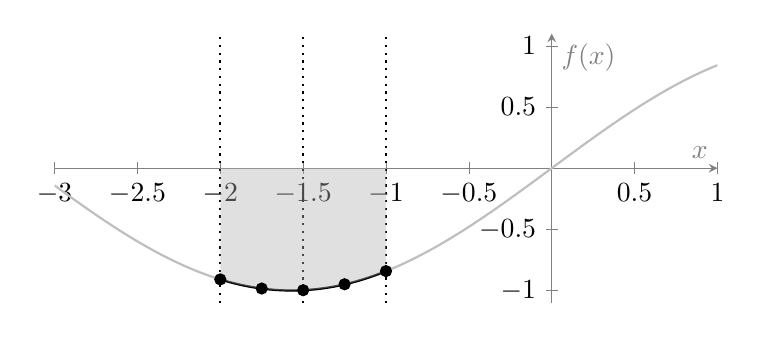
\begin{tikzpicture}
        \begin{axis}[
              width=10cm,
              height=5cm,
              axis x line=middle,
              axis y line=middle,
              xlabel={$x$},
              ylabel={$f(x)$},
              domain=-3:1,
              samples=100,
              ymin=-1.1, ymax=1.1,
              xmin=-3, xmax=1,
              legend style={at={(0.5,-0.2)},anchor=north},
              tick style={gray},
              label style={gray},
              axis line style={gray},
        ]
          % Vertical dotted lines at x=-2, -1.5, -1
          \addplot[dotted, thick, black, domain=-2:-2, samples=2] coordinates {(-2,-1.1) (-2,1.1)};
          \addplot[dotted, thick, black, domain=-1.5:-1.5, samples=2] coordinates {(-1.5,-1.1) (-1.5,1.1)};
          \addplot[dotted, thick, black, domain=-1:-1, samples=2] coordinates {(-1,-1.1) (-1,1.1)};
        % Continuous curve: sin(x) in light gray
        \addplot[gray!50, thick, smooth] {sin(deg(x))};
        % Simpson's rule: quadratic interpolant for [-2, -1.5, -1]
        \addplot[
            black,
            thick,
            domain=-2:-1,
            samples=50,
        ] {(-0.90930)*((x+1.5)*(x+1))/0.5 + (-0.99749)*((x+2)*(x+1))/(-0.25) + (-0.84147)*((x+2)*(x+1.5))/0.5};
        % Fill under the parabola for Simpson's rule on [-2, -1]
        \addplot [
            fill=gray!60, fill opacity=0.4, draw=none,
            domain=-2:-1,
            samples=50
        ] {(-0.90930)*((x+1.5)*(x+1))/0.5 + (-0.99749)*((x+2)*(x+1))/(-0.25) + (-0.84147)*((x+2)*(x+1.5))/0.5} \closedcycle;
        % Endpoints for [-2, -1.5, -1]
        \addplot[black, only marks, mark=*] coordinates {
            (-2, -0.90930)
            (-1.5, -0.99749)
            (-1, -0.84147)
        };
        % Midpoints for Simpson's rule intervals
        \addplot[black, only marks, mark=*] coordinates {
            (-1.75, -0.98363)
            (-1.25, -0.94898)
        };
        \end{axis}
    \end{tikzpicture}
    \caption{Continuous curve $f(x)=\sin(x)$ and Simpson's rule areas (gray, under the parabolas) for $a=-2$, $b=-1.5$, $h=0.5$ and $a=-1.5$, $b=-1$, $h=0.5$. 
    Black dots: endpoints. Black dots: midpoints at $x=-1.75$ and $x=-1.25$. Solid line at $x=-1.5$ separates the two intervals. 
    Each parabola illustrates the quadratic interpolant used by Simpson's rule on its subinterval.}
    \label{fig:simpsonrule}
\end{figure}

\newthought{Lagrange interpolation and quadrature.}
Lagrange interpolation constructs the unique polynomial of degree \(\le n\) that passes through given nodes $\{(x_j,y_j)\}_{j=0}^n$ using the basis
\begin{equation}
L_j(x)=\prod_{\substack{m=0 \\ m\neq j}}^{n} \frac{x - x_m}{x_j - x_m}.
\end{equation}

The general form of a quadratic polynomial is:
\begin{align*}
    f(x) = f(a) \cdot \frac{(x-m)(x-b)}{(a-m)(a-b)} + f(m) \cdot \frac{(x-a)(x-b)}{(m-a)(m-b)} + f(b) \cdot \frac{(x-a)(x-m)}{(b-a)(b-m)}
\end{align*}
\marginnote{\newthought{Try with some points.} Start with $x=0$ and see how the linear factors play out.}


For a symmetric interval, the area under $f(x)$ is best approximated by giving the endpoints weight $h/6$ each and the midpoint weight $2h/3$:
$A = C = h/6$, $B = 2h/3$ - we can verify this by integrating the Lagrange basis polynomials over $[a, b]$ 
and confirming that they yield these weights, but we omit the detailed calculation here.
In a symmetric interval, the nodes are equally spaced: \(x_0=a\), \(x_1=m=\tfrac{a+b}{2}\), \(x_2=b\), so that the midpoint satisfies \(m-a=b-m=h\).

Thus,
\begin{align*}
    \int_a^b f(x) \, dx &\approx \frac{h}{6} f(a) + \frac{2h}{3} f(m) + \frac{h}{6} f(b) \\
    &= \frac{h}{6} [f(a) + 4f(m) + f(b)]
\end{align*}

\newthought{Composite Simpson's Rule} again applies Simpson's rule on each pair of subintervals and 
sums the results (assume $n$ is even and $x_i=a+ih$). Starting from the integral:\\


\begin{align*}
    \int_a^b f(x)\, dx &\approx \sum_{i=0}^{n-1} \int_{x_i}^{x_{i+1}} f(x)\, dx \\
    &\approx \sum_{k=0}^{n/2-1} \frac{h}{6}\bigl[f(x_{2k}) + 4f(x_{2k+1}) + f(x_{2k+2})\bigr]\ \\
    &= \frac{h}{6}\Bigl[f(x_0) + 4\sum_{k=0}^{n/2-1} f(x_{2k+1}) + 2\sum_{k=1}^{n/2-1} f(x_{2k}) + f(x_n)\Bigr] \\
    &= \frac{h}{3}\left[f(x_0) + 4\sum_{\substack{i=1\\ i\ \text{odd}}}^{n-1} f(x_i) + 2\sum_{\substack{i=2\\ i\ \text{even}}}^{n-2} f(x_i) + f(x_n)\right].
\end{align*}
\marginnote{What happens, when you approximate a linear function with a quadratic?} 
\marginnote{\newthought{Runge's phenomenon:} High-degree polynomial interpolation oscillates due to overfitting, leading to large errors at the edges of the interval.}

\iffalse
\newthought{Quadrature rules in general}  
are formulas for approximating definite integrals by weighted sums of function values at specific points (nodes) in the interval. The general form is:
\begin{equation}
    \int_a^b f(x)\,dx \approx \sum_{i=1}^n w_i f(x_i)
\end{equation}
where $x_i$ are the nodes and $w_i$ are the weights. Different quadrature rules choose nodes and weights differently:
Gaussian quadrature is a powerful family of quadrature rules that chooses both the nodes $x_i$ and weights $w_i$ optimally (not equally spaced) to maximize accuracy. For $n$ nodes, Gaussian quadrature is exact for all polynomials up to degree $2n-1$. The most common case is Gauss-Legendre quadrature, which integrates functions on $[-1,1]$ using roots of Legendre polynomials as nodes. Unlike Newton-Cotes rules, Gaussian quadrature achieves much higher accuracy with fewer function evaluations, especially for smooth integrands.
\index{Legendre polynomials}
\newthought{Legendre polynomials} are a sequence of orthogonal polynomials $P_n(x)$ defined on the interval $[-1, 1]$. They satisfy the orthogonality relation:
\[
\int_{-1}^1 P_n(x) P_m(x) \, dx = 0 \quad \text{for } n \neq m
\]
and are solutions to Legendre's differential equation. The first few are:
\begin{align*}
P_0(x) &= 1 \\
P_1(x) &= x \\
P_2(x) &= \frac{1}{2}(3x^2 - 1) \\
P_3(x) &= \frac{1}{2}(5x^3 - 3x)
\end{align*}
In Gauss-Legendre quadrature, the nodes $x_i$ are chosen as the roots of $P_n(x)$.


\begin{equation}
    \int_a^b f(x) \, dx \approx \frac{h}{3}[f(a) + 4f(m) + f(b)]
\end{equation}

where $m = (a+b)/2$ and $h = (b-a)/2$.

\fi


\newthought{Practical advice:} Stop at Simpson. For higher accuracy, use composite rules with more subintervals. 
High-degrees ($n \geq 8$) develop negative weights and become unstable.


\begin{table*}[ht]
\centering
\begin{tabular*}{\textwidth}{@{\extracolsep{\fill}}p{0.33\textwidth}p{0.33\textwidth}p{0.33\textwidth}}
\toprule
\textbf{Method} & \textbf{Single Interval Error} & \textbf{Accumulated Error} \\
\midrule
Left/Right & $O(h^2)$ & $O(h)$ \\
Midpoint & $O(h^3)$ & $O(h^2)$ \\
Trapezoid & $O(h^3)$ & $O(h^2)$ \\
Simpson's 1/3 & $O(h^5)$ & $O(h^4)$ \\
In General (Gaussian Quadrature) & $O(h^{2n})$ & $O(h^{2n-1})$ \\
\bottomrule
\end{tabular*}
\vspace{2em}
\caption{Comparison of quadrature method accuracies. Higher-order methods achieve given accuracy with fewer function evaluations. 
$h$ is the step size, and $n$ is the number of evaluation points for Gaussian quadrature.}
\label{tab:quadrature_comparison}
\end{table*}


\section{Monte Carlo \& the Curse of Dimensionality}
\index{curse of dimensionality} \index{Monte Carlo}

\newthought{For $d$-dimensional integrals,} deterministic quadrature with $N$ points per dimension needs $N^d$ total points.
\marginnote{\newthought{A neural network with} $d = 10^6$ or 1 million parameters 
would need $(N)^{10^6}$ grid points. Even $N = 2$ gives $2^{10^6}$, a number with 300,000 digits.}
There is no way to do this, let alone iterate on it during iterative optimization.



\newthought{Random sampling} allows to estimate the integral without evaluating it on a full grid. 
The integral can be rewritten as an expectation:
\begin{equation}
    I = \int_\Omega f(\mathbf{x}) \, d\mathbf{x} = |\Omega| \cdot \mathbb{E}_{\mathbf{X} \sim \text{Uniform}(\Omega)}[f(\mathbf{X})].
\end{equation}
This identity means the definite integral equals the domain volume times the average value of $f$ under a uniform draw from $\Omega$. Practically this motivates a sampling estimator: draw points uniformly in $\Omega$, compute $f$ at those points, average the results, and multiply by $|\Omega|$ to estimate the integral.

\marginnote{\newthought{$\Omega$} is the domain of integration, and $|\Omega|$ is its length. For a 1D integral over $[a, b]$, we have $|\Omega| = b - a$. For higher dimensions, it's the product of the lengths of each dimension.}

\newthought{Monte Carlo uniform sampling} on $[-2,-1]$.\\
Let $X\sim\mathrm{Uniform}(-2,-1)$. Then \\


\begin{equation}
    I = \frac{|\Omega|}{N} \sum_{i=1}^{N} f(\mathbf{X}_i), \qquad \mathbf{X}_i \stackrel{\text{i.i.d.}}{\sim} \text{Uniform}(\Omega).
\end{equation}



\begin{figure}[h]
    \centering
    % Requires: \usepackage{pgfplots}
    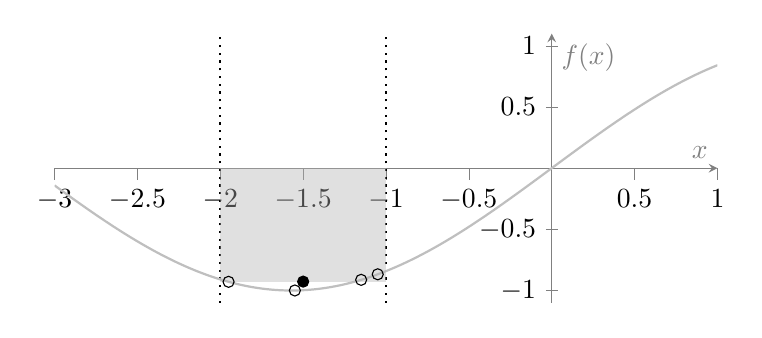
\begin{tikzpicture}
        \begin{axis}[
              width=10cm,
              height=5cm,
              axis x line=middle,
              axis y line=middle,
              xlabel={$x$},
              ylabel={$f(x)$},
              domain=-3:1,
              samples=100,
              ymin=-1.1, ymax=1.1,
              xmin=-3, xmax=1,
              legend style={at={(0.5,-0.2)},anchor=north},
              tick style={gray},
              label style={gray},
              axis line style={gray},
              ybar,
              bar width=0.5,
        ]
                % Vertical dotted guide lines (use axis coordinates to avoid interfering with plots)
                    \draw[dotted, thick, black] (axis cs:-2,-1.1) -- (axis cs:-2,1.1);
                    \draw[dotted, thick, black] (axis cs:-1,-1.1) -- (axis cs:-1,1.1);
        % Continuous curve: sin(x) in light gray
        \addplot[gray!50, thick, smooth] {sin(deg(x))};
        % Gray bar for single midpoint interval (average of MC samples)
        \addplot[ybar, bar width=1, fill=gray!60, fill opacity=0.4, draw=none] coordinates {
            (-1.5, -0.927228)
        };
        % Monte Carlo (random) samples shown as red dots (sample x in [-2,-1])
        \addplot[black, only marks, mark=o] coordinates {
            (-1.95, -0.92895)
            (-1.55, -0.99978)
            (-1.15, -0.91276)
            (-1.05, -0.86742)
        };
        % Average value of the samples shown as a black dot (single midpoint)
        \addplot[black, only marks, mark=*] coordinates {
            (-1.5, -0.927228)
        };
        \end{axis}
    \end{tikzpicture}
    \caption{Continuous curve $f(x)=\sin(x)$ and midpoint rule integrals (gray bars) for $a=-2$, $b=-1$, $h=0.5$. Circles: endpoints.
    The bars now touch, illustrating the midpoint rule without a gap.}
    \label{fig:montecarlo}
\end{figure}

\marginnote{\newthought{Midpoint rule} is a special case of Monte Carlo with $N=1$ sample at the midpoint.}

\newthought{Bias.} Because expectation is linear, this estimator is unbiased, meaning its expected value equals the true integral, for the number of $N \to \infty$:
\begin{equation}
    \mathbb{E}[\hat I_N] = I. 
\end{equation}

\marginnote{\newthought{i.i.d}, independent and identically distributed, means that all $\mathbf{X}_i$ are not correlated and that they all come from the same underlying distribution.}

\newthought{Variance.} The variance, a measure of the spread of the estimator around its mean, or how how large the error of the estimator can be,
follows from independence of the samples:
\begin{equation}
    \mathrm{Var}(\hat I_N) = \frac{|\Omega|^2}{N} \mathrm{Var}\bigl(f(\mathbf{X})\bigr) = \frac{|\Omega|^2 \sigma_f^2}{N},
\end{equation}

where $\sigma_f^2 = \mathrm{Var}(f(\mathbf{X}))$. Hence the standard error is

\begin{equation}
    \mathrm{SE}(\hat I_N) = \frac{|\Omega|\,\sigma_f}{\sqrt{N}}.
\end{equation}

% TODO: Make the break-even dimension between grid quadrature and Monte
% Carlo explicit. For a $d$-dimensional grid with $N$ total evaluations,
% the per-axis spacing is $h = N^{-1/d}$, so a second-order rule
% (midpoint, trapez) yields error $O(h^2) = O(N^{-2/d})$. Setting this
% equal to the Monte Carlo rate $O(N^{-1/2})$ gives $2/d = 1/2$, hence
% $d = 4$. Currently the chapter says only "MC is attractive in high
% dimensions" qualitatively; the concrete break-even at $d \approx 4$
% should be added (e.g. as a worked margin note here) so that exam
% questions asking for the crossover dimension are answerable purely
% from the script. Referenced by exam_01 2(c).
\newthought{Dimension independent.}
It is trivial to see, that for large $N$ the sampling error converges with, $O(1/\sqrt{N})$ for Monte Carlo, which makes it attractive in high dimensions.
Quadrature rules outperform in terms of their convergence rates, but the convergence effort explodes with the dimension, as we need $N^d$ points to maintain the same accuracy.

\begin{marginfigure}
    \centering
    \includegraphics[width=\marginparwidth]{figures/batchnoise.png}
    \caption{Effect of batch size on gradient noise: smaller batches produce larger variance 
    (showing up in the width of the training loss band) in the gradient estimate 
    (Source: \href{https://cs231n.github.io/neural-networks-3/\#baby}{Stanford CS231n Note}).}
    \label{fig:batchnoise}
\end{marginfigure}
\marginnote{As a beneficial side effect, computational cost is $n/b$ times cheaper per update step. 
For $n = 10^6$, and $b = 100$: SGD does 10,000 iterations with the compute GD needs for 1.}

\newthought{Convergence in SGD.} Mini-batch gradients used in SGD are Monte Carlo estimates of the true gradient, based on a samples drawn into a batch.
Increasing the batch size reduces variance roughly by $1/b$, directly analogous to the $1/N$ variance scaling above. 
This connection explains why batch size controls the noise–variance trade-off in training.



















% ==============================================================================================
% STUDENT ACTIVATION BLOCK

\newpage
\section{Examples \& Exercises}
\index{exercises}


\newthought{Let's stick} to our example from the methods sections, and calculate the integral of $\sin(x)$ from $-2$ to $-1$ 
using different methods. In order to be able to quantify the error of each method, we need the exact value. So let's compute the exact value of the integral:
\begin{align*}
        \tilde{I} &= \int_{-2}^{-1} \sin(x)\,dx \\
            &= [-\cos(x)]_{-2}^{-1} \\
            &= -\cos(-1) + \cos(-2) \\
            &\approx -0.9564491424.
\end{align*}

\newthought{Midpoint rule by hand.} Compute $\int_{-2}^{-1} \sin(x) dx$ using the midpoint rule with $n=1$ interval.
The midpoint is $m = (-2 + (-1))/2 = -1.5$, so the midpoint rule gives us:
\begin{align*}
    \hat{I} &\approx (b - a) \cdot f(m) \\
      &= 1 \cdot \sin(-1.5) \\
      &\approx -0.99749.
\end{align*}
The error is $|\tilde{I} - \hat{I}| \approx 0.04104$, which is the small difference between the midpoint estimate and the true value.

\marginnote{\newthought{Further things worth trying} are to calculate the approximation on the endpoints of the interval, comparing the error.}

\newthought{Midpoint rule with more intervals.} Now compute the midpoint rule with $n=2$ intervals, which means we will have two midpoints at $-1.75$ and $-1.25$.
This gives us: 
\begin{align*}
    h &= 0.5 \\
    \hat{I} &\approx h \cdot [f(-1.75) + f(-1.25)] \\
      &= 0.5 \cdot [\sin(-1.75) + \sin(-1.25)] \\
      &\approx -0.927228.
\end{align*}
The error is $|\tilde{I} - \hat{I}| \approx 0.02922$, which is smaller than the error with $n=1$ interval, illustrating how composites, or increasing the number of intervals improves the approximation.


\newthought{Trapezoid by hand.}
Use the trapezoid rule to compute $\int_{-2}^{-1} \sin(x) dx$ with $n=2$ intervals.
The endpoints are $-2$, $-1.5$, and $-1$. The trapezoid rule gives us:
\begin{align*}
    h &= 0.5 \\
    T_2 &= \frac{h}{2} [f(-2) + 2f(-1.5) + f(-1)] \\
        &= 0.25 \cdot [-0.90930 + 2(-0.99749) + (-0.84147)] \\
        &\approx -0.927228.
\end{align*}
The error is the same as the midpoint rule with $n=2$ intervals, which is not necessarily a coincidence, as both methods are second-order accurate and can yield similar results for certain functions and interval choices.




\vspace{2em}
\newthought{Simpson's rule by hand.} Use Simpson's rule to compute $\int_{-2}^{-1} \sin(x) dx$ with $n=2$ intervals.
The endpoints are $-2$, $-1.5$, and $-1$. Simpson's rule gives us:
\begin{align*}
    h &= 0.5 \\
    S_2 &= \frac{h}{3} [f(-2) + 4f(-1.5) + f(-1)] \\
        &= \frac{0.5}{3} \cdot [-0.90930 + 4(-0.99749) + (-0.84147)] \\
        &\approx -0.9564491424.
\end{align*}
The error is $|\tilde{I} - S_2| \approx 0.0000000000$, which is essentially zero, illustrating that Simpson's rule is exact for this particular integral, as $\sin(x)$ can be well approximated by a quadratic polynomial over the interval $[-2, -1]$.


\marginnote{\newthought{Try with more intervals,} see how the error decreases and check whether you know your way around composites in Simpson's and Trapezoid rules.}


\newthought{Monte Carlo by hand.} Use Monte Carlo estimation to compute $\int_{-2}^{-1} \sin(x) dx$ with $N=4$ random samples, 
which is similar to the compute efforts of the trapezoid method. Let's assume the random samples are: 
\begin{align*}
    X_1 &= -1.95, \quad f(X_1) = \sin(-1.95) \approx -0.92895, \\
    X_2 &= -1.55, \quad f(X_2) = \sin(-1.55) \approx -0.99978, \\
    X_3 &= -1.15, \quad f(X_3) = \sin(-1.15) \approx -0.91276, \\
    X_4 &= -1.05, \quad f(X_4) = \sin(-1.05) \approx -0.86742.
\end{align*}

The Monte Carlo estimate is:
\begin{align*}
    \hat{I} &= (b - a) \cdot \frac{1}{N} \sum_{i=1}^{N} f(X_i) \\
            &= 1 \cdot \frac{1}{4} (-0.92895 - 0.99978 - 0.91276 - 0.86742) \\
            &\approx -0.927228.
\end{align*}
The error is $|\tilde{I} - \hat{I}| \approx 0.02922$, which is the same as the midpoint method. 



\newthought{alternative error estimation for Monte Carlo.} For our concrete example with $N=4$ and the sample mean of
\(\bar f \approx -0.927228\). Using the unbiased sample variance estimator:
\begin{equation}
    Var(f(\mathbf{X})) = \frac{1}{N-1} \sum_{i=1}^N (f(X_i) - \bar f)^2.
\end{equation}

We obtain the sample variance and standard error of the Monte Carlo estimator as follows:
\begin{align*}
    \sigma_f^2 &= Var(f(\mathbf{X}))  \\ 
               &\approx 0.003036, \\
    \sigma_{f} &\approx 0.05512, \\
    \mathrm{SE}(\hat I_N) &\approx \frac{|\Omega|\, \sigma_f}{\sqrt{N}} \\
    &= \frac{1\cdot 0.05512}{2} \\
    &\approx 0.02756.
\end{align*}

What happens if we increase $N$ to 16? 
The error should decrease by a factor of 2, since the standard error scales as $1/\sqrt{N}$.
Briefly elaborate on how the error of the Monte Carlo estimator is dimension independant.






\vspace{2em}
\marginnote{\newthought{Code} can be found at \url{https://github.com/Quillstacks/lecturecode_numericalmethods.git}.}
\newthought{Enter higher dimensions on your machine.} Implement Monte Carlo integration for a $d$-dimensional integral, 
such as integrating a multivariate Gaussian function over a hypercube. While slowly increasing $d$, observe how the error behaves for different methods.
Even more, observe how grid-based quadrature methods become infeasible in terms of computational cost as $d$ grows.
Optionally, see how similar effects arise in optimization by implementing gradient descent and mini-batch
stochastic gradient descent on a high-dimensional function. Only watch compute times.


\vfill
\section{Self-Reflection and Recap}
\index{recap}

\newthought{Self-Reflection} Questions to guide your understanding:
\begin{itemize}
    \item How does the error of the midpoint, trapezoid, Simpson's rule and Monte Carlo compare?
    \item Why has the midpoint rule better accuracy than the left or right endpoint rules?
    \item How does composite methods improve accuracy, and what is the trade-off?
    \item Why do deterministic quadrature methods fail in high dimensions?
    \item In which way, is the midpoint rule a special case of Monte Carlo estimation?
    \item What is the intuition behind Monte Carlo not exploding in high dimensions?
    \item When would you use Simpson's rule vs.\ Monte Carlo?
    \item How is the mini-batch mean in SGD related to Monte Carlo estimation?
    \item How does the gradient estimation in SGD help escape local minima?
\end{itemize}

\newthought{Recap} of Key Concepts:
\begin{itemize}
    \item Deterministic quadrature methods (midpoint, trapezoid, Simpson's) approximate integrals using weighted sums of function values at 
    specific points. They are accurate and converge fast for smooth, low-dimensional problems.
    \item Monte Carlo integration estimates integrals by averaging function values at random samples. 
    It is unbiased and has a convergence rate of $O(1/\sqrt{N})$, making it independent of the dimensionality of the problem.
    \item In SGD, mini-batch gradients are Monte Carlo estimates of the true gradient.
\end{itemize}



\marginnote{\newthought{Teaser.} Are these six chapters really six things?}

\newthought{Six chapters in,} we have learned to represent numbers, reason about error,
find roots, optimize, integrate, and sample.
These felt like distinct topics.
In the next chapter, we will run them all once on one small dataset, and we will notice that they were facets of a single workflow all along: fitting a model to data.

%%%%%%%%%%%%%%%%%%%%%%%%%%%%%%%%%%%%%%%%%%%%%%%%%%%%%%%%%%%%%%%%%%%%%%%%%%%%%%
